\section{Results Discussion of The Battery Modeling}
The results from the power analyzer have been satisfactory and the robustness of the power analyzer architecture allows for the simulation of various BMS tests, such as low battery voltage, high battery voltage protection, and soc estimation.
Batteries can be imbalanced for testing different battery balancing algorithms in the battery pack module by passing different initial SoC values. In the practical sense, low and high battery voltage testing takes tons of time with batteries. Achieving fast charging and discharging with the batteries needs a high sink/source current, which could be a limitation in many instruments. Thanks to the PowerAnalyzer, it allows emulating fast charging and discharging of batteries by adding some bias current(only added in the script) with the actual current that is flowing in the battery emulator. The actual battery emulator does not know anything it is not smart enough to realize what is going on with the current flowing in the system. On contrary, the script can emulate this behavior and set a new terminal voltage to each channel of the battery emulator, every time the PowerAnalyzer sample the current flowing in the battery emulator.

The following code, snippet illustrates the biased current simulation. "$currents = self.batEmulator.BateryEmulatorCellCurrent$" will fetch the actual current that is flowing in the battery emulator; for the "$currents$" array the "$ibattBias$" biased current is added and calculated as new open circuit voltage "$batEmulator.batteryEmulatorVoltageSet(cellNo=i,cellVoltage=VOC)$", and SoC is the updated open circuit voltage set to the battery emulator terminal voltage(each channel respectively).
\begin{lstlisting}[language=Python, caption=Emulating Sudo BiasCurrent in the PowerAnalyzer ]
    def batVoltageSOC(self):
        batVoltSOC =dict()
        currents = self.batEmulator.BateryEmulatorCellCurrent
        
        biasedCurrent = []
        # print(f'Current that flowinf in Chroma {currents}')
        
        #add the sudo bias current 
        for i in range(0,len(self.SOC0)):
            biasedCurrent.append(currents[i]+self.ibattBias)
                
        for i in range(0,len(self.SOC0)):
            [batVlot,VOC] = self.Batt[i].battVoltage(biasedCurrent[i])
            batVoltSOC[batVlot] = self.Batt[i].CoulombSOC
            self.batEmulator.batteryEmulatorVoltageSet(cellNo=i,
                                    cellVoltage=VOC)
            
        return batVoltSOC
\end{lstlisting}

% \begin{figure}[h]
% 	\centering
% 	\subfigure[Single Battery Charging (blue)/Discharging (orange) Voltage  Vs Cycles]{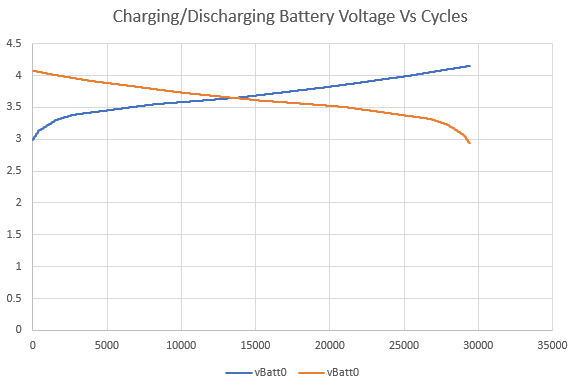
\includegraphics[scale=.5]{Chap06/Figures/Singlebatt_charge_discharge_voltage.PNG}}
% 	\qquad
% 	\subfigure[Single Battery Charging (blue)/Discharging (orange) SoC  Vs Cycles]{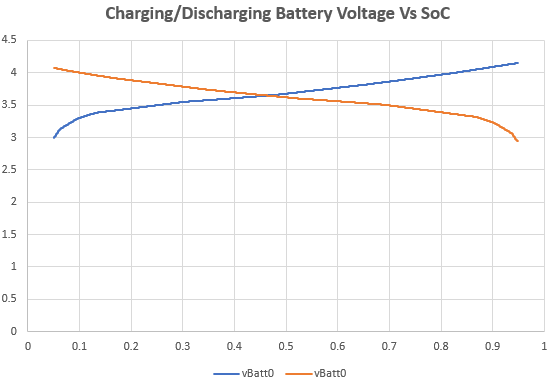
\includegraphics[scale=.5]{Chap06/Figures/Singlebatt_charge_discharge_voltage_SoC.PNG}}
% 	\qquad
% 	\subfigure[Single Battery Charging (blue)/Discharging (orange) Voltage  Vs SoC]{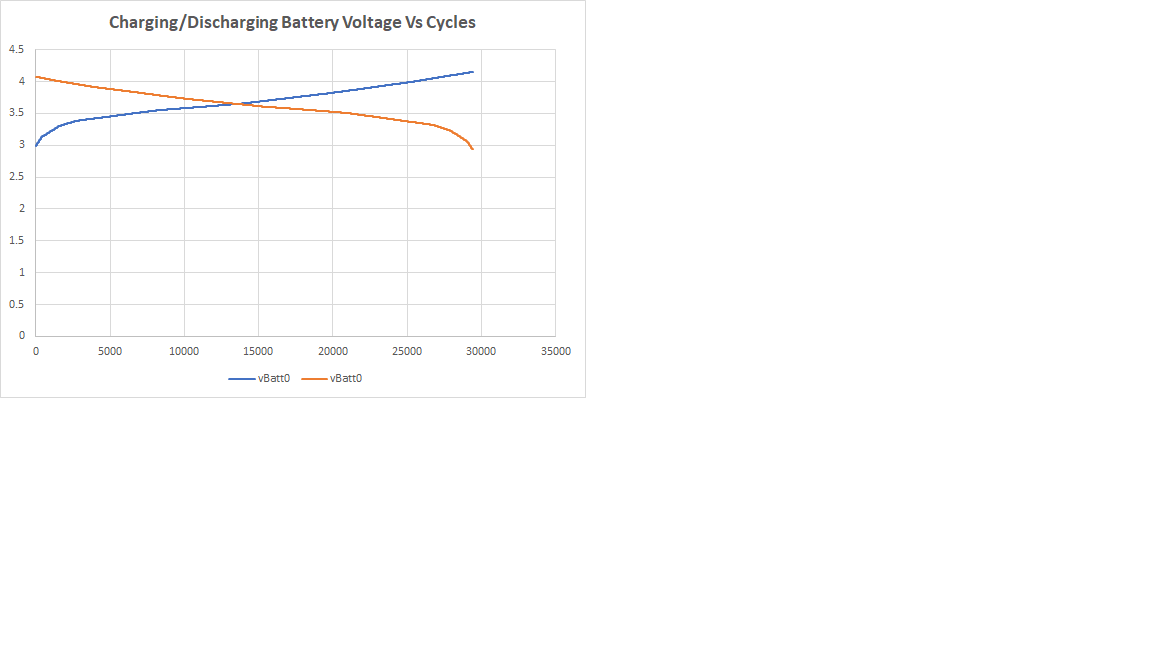
\includegraphics[scale=.5]{Chap06/Figures/Untitled.png}}
% 	\caption{Single Battery Charging and Discharging Behavior}
% 	\label{fig:Single_Batt_charge_discharge}
% \end{figure}



% \begin{tikzpicture}
%     \begin{axis}[scale only axis, xlabel = x, ylabel = y,  ytick pos=left]
%     \addplot table[x=x,y=y] {./Chap06/Code/test.xlsx};
%      \end{axis}
% \end{tikzpicture}


% % This file was created with tikzplotlib v0.10.1.
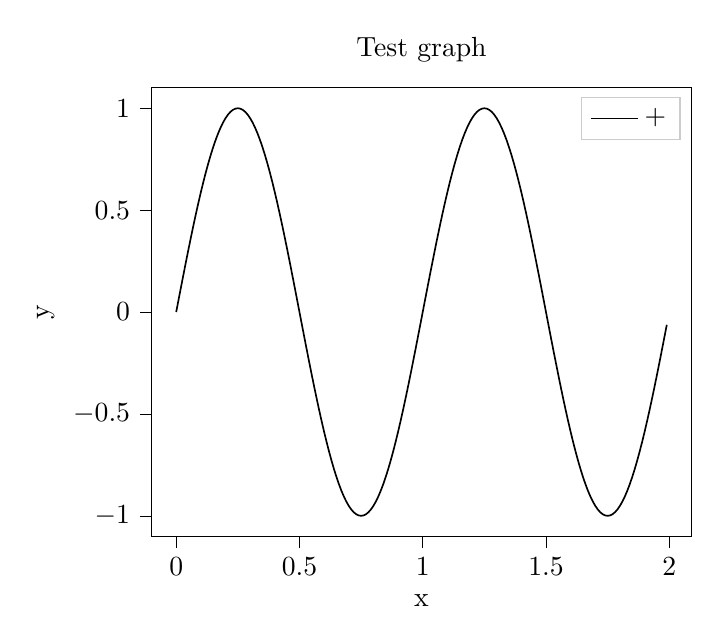
\begin{tikzpicture}

\definecolor{darkgray176}{RGB}{176,176,176}
\definecolor{lightgray204}{RGB}{204,204,204}

\begin{axis}[
legend cell align={left},
legend style={fill opacity=0.8, draw opacity=1, text opacity=1, draw=lightgray204},
tick align=outside,
tick pos=left,
title={Test graph},
x grid style={darkgray176},
xlabel={x},
xmin=-0.0995, xmax=2.0895,
xtick style={color=black},
y grid style={darkgray176},
ylabel={y},
ymin=-1.1, ymax=1.1,
ytick style={color=black}
]
\addplot [semithick, black]
table {%
0 0
0.01 0.0627905195293134
0.02 0.125333233564304
0.03 0.187381314585725
0.04 0.248689887164855
0.05 0.309016994374947
0.06 0.368124552684678
0.07 0.425779291565073
0.08 0.481753674101715
0.09 0.535826794978997
0.1 0.587785252292473
0.11 0.63742398974869
0.12 0.684547105928689
0.13 0.728968627421412
0.14 0.770513242775789
0.15 0.809016994374947
0.16 0.844327925502015
0.17 0.876306680043864
0.18 0.90482705246602
0.19 0.929776485888251
0.2 0.951056516295154
0.21 0.968583161128631
0.22 0.982287250728689
0.23 0.992114701314478
0.24 0.998026728428272
0.25 1
0.26 0.998026728428272
0.27 0.992114701314478
0.28 0.982287250728689
0.29 0.968583161128631
0.3 0.951056516295154
0.31 0.929776485888251
0.32 0.904827052466019
0.33 0.876306680043863
0.34 0.844327925502015
0.35 0.809016994374947
0.36 0.770513242775789
0.37 0.728968627421411
0.38 0.684547105928689
0.39 0.63742398974869
0.4 0.587785252292473
0.41 0.535826794978997
0.42 0.481753674101716
0.43 0.425779291565073
0.44 0.368124552684678
0.45 0.309016994374948
0.46 0.248689887164855
0.47 0.187381314585725
0.48 0.125333233564305
0.49 0.0627905195293136
0.5 1.22464679914735e-16
0.51 -0.0627905195293133
0.52 -0.125333233564304
0.53 -0.187381314585725
0.54 -0.248689887164855
0.55 -0.309016994374948
0.56 -0.368124552684678
0.57 -0.425779291565073
0.58 -0.481753674101715
0.59 -0.535826794978996
0.6 -0.587785252292473
0.61 -0.63742398974869
0.62 -0.684547105928689
0.63 -0.728968627421411
0.64 -0.770513242775789
0.65 -0.809016994374947
0.66 -0.844327925502015
0.67 -0.876306680043864
0.68 -0.90482705246602
0.69 -0.929776485888251
0.7 -0.951056516295154
0.71 -0.968583161128631
0.72 -0.982287250728689
0.73 -0.992114701314478
0.74 -0.998026728428272
0.75 -1
0.76 -0.998026728428272
0.77 -0.992114701314478
0.78 -0.982287250728689
0.79 -0.968583161128631
0.8 -0.951056516295154
0.81 -0.929776485888251
0.82 -0.90482705246602
0.83 -0.876306680043863
0.84 -0.844327925502016
0.85 -0.809016994374948
0.86 -0.77051324277579
0.87 -0.728968627421412
0.88 -0.684547105928689
0.89 -0.63742398974869
0.9 -0.587785252292473
0.91 -0.535826794978996
0.92 -0.481753674101715
0.93 -0.425779291565072
0.94 -0.368124552684678
0.95 -0.309016994374948
0.96 -0.248689887164855
0.97 -0.187381314585725
0.98 -0.125333233564305
0.99 -0.0627905195293133
1 -2.44929359829471e-16
1.01 0.0627905195293128
1.02 0.125333233564304
1.03 0.187381314585724
1.04 0.248689887164855
1.05 0.309016994374947
1.06 0.368124552684678
1.07 0.425779291565073
1.08 0.481753674101716
1.09 0.535826794978997
1.1 0.587785252292474
1.11 0.63742398974869
1.12 0.684547105928689
1.13 0.728968627421412
1.14 0.770513242775789
1.15 0.809016994374948
1.16 0.844327925502015
1.17 0.876306680043863
1.18 0.904827052466019
1.19 0.929776485888251
1.2 0.951056516295154
1.21 0.968583161128631
1.22 0.982287250728689
1.23 0.992114701314478
1.24 0.998026728428272
1.25 1
1.26 0.998026728428272
1.27 0.992114701314478
1.28 0.982287250728689
1.29 0.968583161128631
1.3 0.951056516295154
1.31 0.929776485888252
1.32 0.904827052466019
1.33 0.876306680043863
1.34 0.844327925502015
1.35 0.809016994374948
1.36 0.770513242775789
1.37 0.728968627421411
1.38 0.684547105928688
1.39 0.63742398974869
1.4 0.587785252292473
1.41 0.535826794978997
1.42 0.481753674101716
1.43 0.425779291565074
1.44 0.368124552684678
1.45 0.309016994374948
1.46 0.248689887164855
1.47 0.187381314585726
1.48 0.125333233564304
1.49 0.0627905195293134
1.5 3.67394039744206e-16
1.51 -0.0627905195293127
1.52 -0.125333233564303
1.53 -0.187381314585725
1.54 -0.248689887164855
1.55 -0.309016994374947
1.56 -0.368124552684677
1.57 -0.425779291565073
1.58 -0.481753674101716
1.59 -0.535826794978997
1.6 -0.587785252292473
1.61 -0.637423989748691
1.62 -0.684547105928689
1.63 -0.728968627421412
1.64 -0.770513242775789
1.65 -0.809016994374947
1.66 -0.844327925502016
1.67 -0.876306680043863
1.68 -0.904827052466019
1.69 -0.929776485888251
1.7 -0.951056516295153
1.71 -0.968583161128631
1.72 -0.982287250728688
1.73 -0.992114701314478
1.74 -0.998026728428272
1.75 -1
1.76 -0.998026728428272
1.77 -0.992114701314478
1.78 -0.982287250728689
1.79 -0.968583161128631
1.8 -0.951056516295154
1.81 -0.929776485888252
1.82 -0.904827052466019
1.83 -0.876306680043863
1.84 -0.844327925502015
1.85 -0.809016994374948
1.86 -0.770513242775789
1.87 -0.728968627421411
1.88 -0.684547105928689
1.89 -0.63742398974869
1.9 -0.587785252292473
1.91 -0.535826794978996
1.92 -0.481753674101716
1.93 -0.425779291565074
1.94 -0.368124552684678
1.95 -0.309016994374948
1.96 -0.248689887164856
1.97 -0.187381314585726
1.98 -0.125333233564304
1.99 -0.0627905195293135
};
\addlegendentry{+}
\end{axis}

\end{tikzpicture}

% \begin{figure}[h]
%     \begin{center}
%         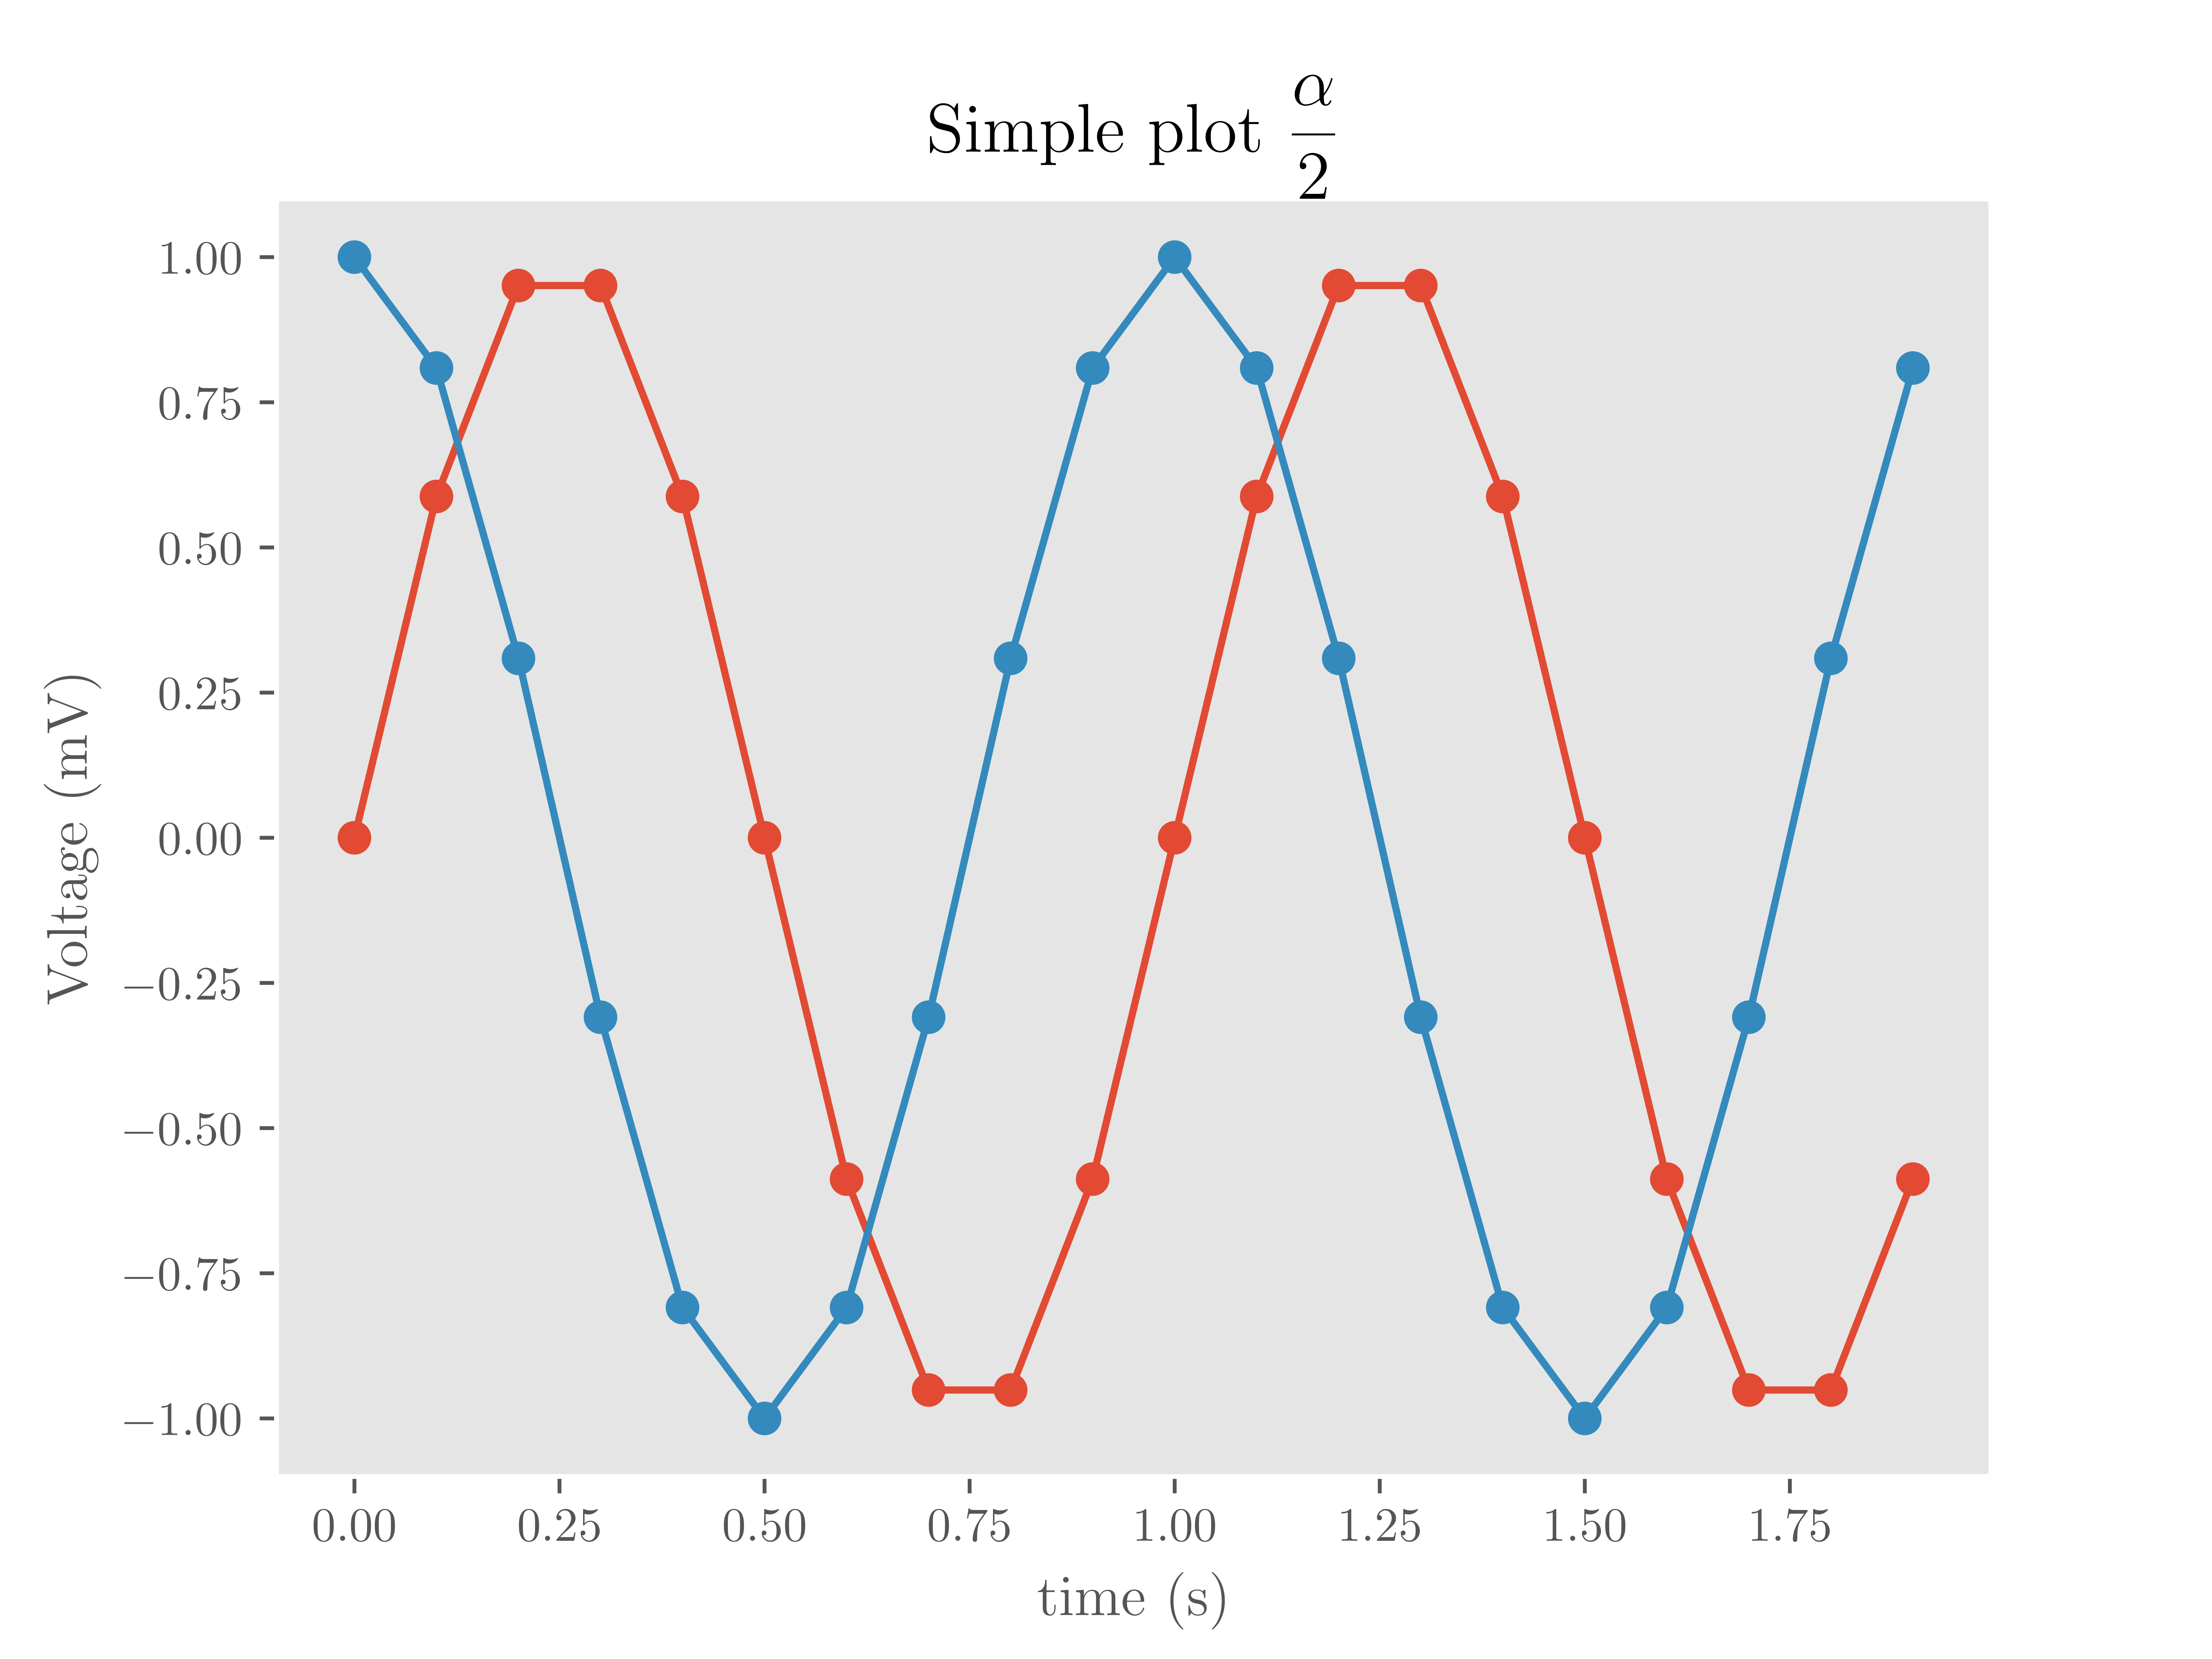
\includegraphics[width=1\textwidth]{Chap06/Code/test.png}
%     \end{center}
%     \caption{A PGF histogram from \texttt{matplotlib}.}
% \end{figure}

% This file was created with tikzplotlib v0.10.1.


\begin{figure}
    \centering
    \resizebox{0.8\textwidth}{!}{% This file was created with tikzplotlib v0.10.1.
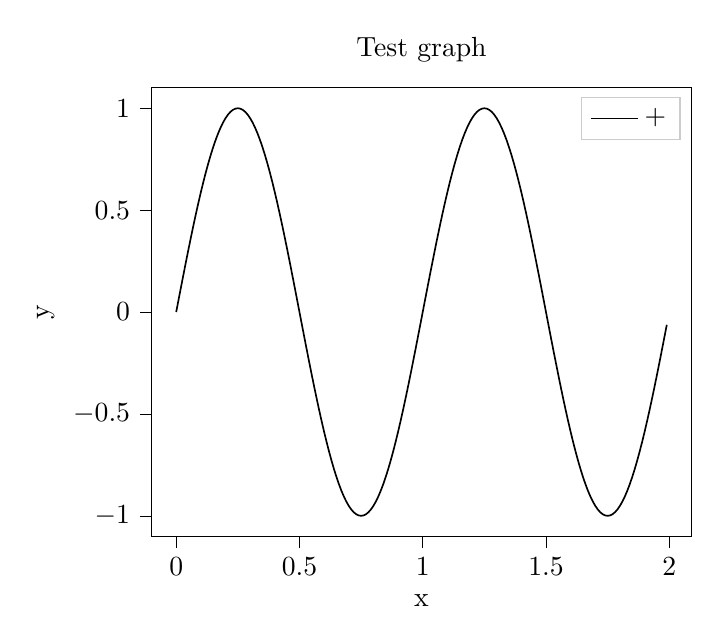
\begin{tikzpicture}

\definecolor{darkgray176}{RGB}{176,176,176}
\definecolor{lightgray204}{RGB}{204,204,204}

\begin{axis}[
legend cell align={left},
legend style={fill opacity=0.8, draw opacity=1, text opacity=1, draw=lightgray204},
tick align=outside,
tick pos=left,
title={Test graph},
x grid style={darkgray176},
xlabel={x},
xmin=-0.0995, xmax=2.0895,
xtick style={color=black},
y grid style={darkgray176},
ylabel={y},
ymin=-1.1, ymax=1.1,
ytick style={color=black}
]
\addplot [semithick, black]
table {%
0 0
0.01 0.0627905195293134
0.02 0.125333233564304
0.03 0.187381314585725
0.04 0.248689887164855
0.05 0.309016994374947
0.06 0.368124552684678
0.07 0.425779291565073
0.08 0.481753674101715
0.09 0.535826794978997
0.1 0.587785252292473
0.11 0.63742398974869
0.12 0.684547105928689
0.13 0.728968627421412
0.14 0.770513242775789
0.15 0.809016994374947
0.16 0.844327925502015
0.17 0.876306680043864
0.18 0.90482705246602
0.19 0.929776485888251
0.2 0.951056516295154
0.21 0.968583161128631
0.22 0.982287250728689
0.23 0.992114701314478
0.24 0.998026728428272
0.25 1
0.26 0.998026728428272
0.27 0.992114701314478
0.28 0.982287250728689
0.29 0.968583161128631
0.3 0.951056516295154
0.31 0.929776485888251
0.32 0.904827052466019
0.33 0.876306680043863
0.34 0.844327925502015
0.35 0.809016994374947
0.36 0.770513242775789
0.37 0.728968627421411
0.38 0.684547105928689
0.39 0.63742398974869
0.4 0.587785252292473
0.41 0.535826794978997
0.42 0.481753674101716
0.43 0.425779291565073
0.44 0.368124552684678
0.45 0.309016994374948
0.46 0.248689887164855
0.47 0.187381314585725
0.48 0.125333233564305
0.49 0.0627905195293136
0.5 1.22464679914735e-16
0.51 -0.0627905195293133
0.52 -0.125333233564304
0.53 -0.187381314585725
0.54 -0.248689887164855
0.55 -0.309016994374948
0.56 -0.368124552684678
0.57 -0.425779291565073
0.58 -0.481753674101715
0.59 -0.535826794978996
0.6 -0.587785252292473
0.61 -0.63742398974869
0.62 -0.684547105928689
0.63 -0.728968627421411
0.64 -0.770513242775789
0.65 -0.809016994374947
0.66 -0.844327925502015
0.67 -0.876306680043864
0.68 -0.90482705246602
0.69 -0.929776485888251
0.7 -0.951056516295154
0.71 -0.968583161128631
0.72 -0.982287250728689
0.73 -0.992114701314478
0.74 -0.998026728428272
0.75 -1
0.76 -0.998026728428272
0.77 -0.992114701314478
0.78 -0.982287250728689
0.79 -0.968583161128631
0.8 -0.951056516295154
0.81 -0.929776485888251
0.82 -0.90482705246602
0.83 -0.876306680043863
0.84 -0.844327925502016
0.85 -0.809016994374948
0.86 -0.77051324277579
0.87 -0.728968627421412
0.88 -0.684547105928689
0.89 -0.63742398974869
0.9 -0.587785252292473
0.91 -0.535826794978996
0.92 -0.481753674101715
0.93 -0.425779291565072
0.94 -0.368124552684678
0.95 -0.309016994374948
0.96 -0.248689887164855
0.97 -0.187381314585725
0.98 -0.125333233564305
0.99 -0.0627905195293133
1 -2.44929359829471e-16
1.01 0.0627905195293128
1.02 0.125333233564304
1.03 0.187381314585724
1.04 0.248689887164855
1.05 0.309016994374947
1.06 0.368124552684678
1.07 0.425779291565073
1.08 0.481753674101716
1.09 0.535826794978997
1.1 0.587785252292474
1.11 0.63742398974869
1.12 0.684547105928689
1.13 0.728968627421412
1.14 0.770513242775789
1.15 0.809016994374948
1.16 0.844327925502015
1.17 0.876306680043863
1.18 0.904827052466019
1.19 0.929776485888251
1.2 0.951056516295154
1.21 0.968583161128631
1.22 0.982287250728689
1.23 0.992114701314478
1.24 0.998026728428272
1.25 1
1.26 0.998026728428272
1.27 0.992114701314478
1.28 0.982287250728689
1.29 0.968583161128631
1.3 0.951056516295154
1.31 0.929776485888252
1.32 0.904827052466019
1.33 0.876306680043863
1.34 0.844327925502015
1.35 0.809016994374948
1.36 0.770513242775789
1.37 0.728968627421411
1.38 0.684547105928688
1.39 0.63742398974869
1.4 0.587785252292473
1.41 0.535826794978997
1.42 0.481753674101716
1.43 0.425779291565074
1.44 0.368124552684678
1.45 0.309016994374948
1.46 0.248689887164855
1.47 0.187381314585726
1.48 0.125333233564304
1.49 0.0627905195293134
1.5 3.67394039744206e-16
1.51 -0.0627905195293127
1.52 -0.125333233564303
1.53 -0.187381314585725
1.54 -0.248689887164855
1.55 -0.309016994374947
1.56 -0.368124552684677
1.57 -0.425779291565073
1.58 -0.481753674101716
1.59 -0.535826794978997
1.6 -0.587785252292473
1.61 -0.637423989748691
1.62 -0.684547105928689
1.63 -0.728968627421412
1.64 -0.770513242775789
1.65 -0.809016994374947
1.66 -0.844327925502016
1.67 -0.876306680043863
1.68 -0.904827052466019
1.69 -0.929776485888251
1.7 -0.951056516295153
1.71 -0.968583161128631
1.72 -0.982287250728688
1.73 -0.992114701314478
1.74 -0.998026728428272
1.75 -1
1.76 -0.998026728428272
1.77 -0.992114701314478
1.78 -0.982287250728689
1.79 -0.968583161128631
1.8 -0.951056516295154
1.81 -0.929776485888252
1.82 -0.904827052466019
1.83 -0.876306680043863
1.84 -0.844327925502015
1.85 -0.809016994374948
1.86 -0.770513242775789
1.87 -0.728968627421411
1.88 -0.684547105928689
1.89 -0.63742398974869
1.9 -0.587785252292473
1.91 -0.535826794978996
1.92 -0.481753674101716
1.93 -0.425779291565074
1.94 -0.368124552684678
1.95 -0.309016994374948
1.96 -0.248689887164856
1.97 -0.187381314585726
1.98 -0.125333233564304
1.99 -0.0627905195293135
};
\addlegendentry{+}
\end{axis}

\end{tikzpicture}
}
\end{figure}

\begin{figure}[h]
	\centering
	\subfigure[MIFA antenna Gain Radiation pattern $@ \phi =90\deg$]{\resizebox{0.8\textwidth}{!}{% This file was created with tikzplotlib v0.10.1.
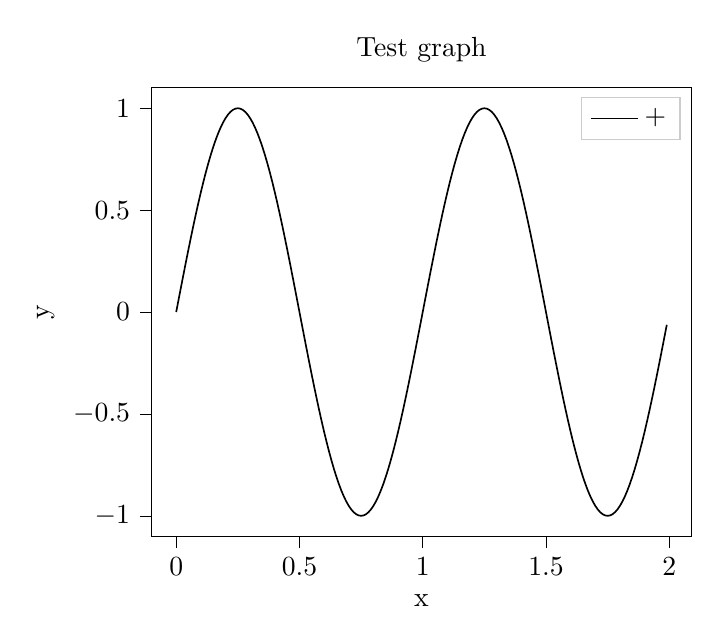
\begin{tikzpicture}

\definecolor{darkgray176}{RGB}{176,176,176}
\definecolor{lightgray204}{RGB}{204,204,204}

\begin{axis}[
legend cell align={left},
legend style={fill opacity=0.8, draw opacity=1, text opacity=1, draw=lightgray204},
tick align=outside,
tick pos=left,
title={Test graph},
x grid style={darkgray176},
xlabel={x},
xmin=-0.0995, xmax=2.0895,
xtick style={color=black},
y grid style={darkgray176},
ylabel={y},
ymin=-1.1, ymax=1.1,
ytick style={color=black}
]
\addplot [semithick, black]
table {%
0 0
0.01 0.0627905195293134
0.02 0.125333233564304
0.03 0.187381314585725
0.04 0.248689887164855
0.05 0.309016994374947
0.06 0.368124552684678
0.07 0.425779291565073
0.08 0.481753674101715
0.09 0.535826794978997
0.1 0.587785252292473
0.11 0.63742398974869
0.12 0.684547105928689
0.13 0.728968627421412
0.14 0.770513242775789
0.15 0.809016994374947
0.16 0.844327925502015
0.17 0.876306680043864
0.18 0.90482705246602
0.19 0.929776485888251
0.2 0.951056516295154
0.21 0.968583161128631
0.22 0.982287250728689
0.23 0.992114701314478
0.24 0.998026728428272
0.25 1
0.26 0.998026728428272
0.27 0.992114701314478
0.28 0.982287250728689
0.29 0.968583161128631
0.3 0.951056516295154
0.31 0.929776485888251
0.32 0.904827052466019
0.33 0.876306680043863
0.34 0.844327925502015
0.35 0.809016994374947
0.36 0.770513242775789
0.37 0.728968627421411
0.38 0.684547105928689
0.39 0.63742398974869
0.4 0.587785252292473
0.41 0.535826794978997
0.42 0.481753674101716
0.43 0.425779291565073
0.44 0.368124552684678
0.45 0.309016994374948
0.46 0.248689887164855
0.47 0.187381314585725
0.48 0.125333233564305
0.49 0.0627905195293136
0.5 1.22464679914735e-16
0.51 -0.0627905195293133
0.52 -0.125333233564304
0.53 -0.187381314585725
0.54 -0.248689887164855
0.55 -0.309016994374948
0.56 -0.368124552684678
0.57 -0.425779291565073
0.58 -0.481753674101715
0.59 -0.535826794978996
0.6 -0.587785252292473
0.61 -0.63742398974869
0.62 -0.684547105928689
0.63 -0.728968627421411
0.64 -0.770513242775789
0.65 -0.809016994374947
0.66 -0.844327925502015
0.67 -0.876306680043864
0.68 -0.90482705246602
0.69 -0.929776485888251
0.7 -0.951056516295154
0.71 -0.968583161128631
0.72 -0.982287250728689
0.73 -0.992114701314478
0.74 -0.998026728428272
0.75 -1
0.76 -0.998026728428272
0.77 -0.992114701314478
0.78 -0.982287250728689
0.79 -0.968583161128631
0.8 -0.951056516295154
0.81 -0.929776485888251
0.82 -0.90482705246602
0.83 -0.876306680043863
0.84 -0.844327925502016
0.85 -0.809016994374948
0.86 -0.77051324277579
0.87 -0.728968627421412
0.88 -0.684547105928689
0.89 -0.63742398974869
0.9 -0.587785252292473
0.91 -0.535826794978996
0.92 -0.481753674101715
0.93 -0.425779291565072
0.94 -0.368124552684678
0.95 -0.309016994374948
0.96 -0.248689887164855
0.97 -0.187381314585725
0.98 -0.125333233564305
0.99 -0.0627905195293133
1 -2.44929359829471e-16
1.01 0.0627905195293128
1.02 0.125333233564304
1.03 0.187381314585724
1.04 0.248689887164855
1.05 0.309016994374947
1.06 0.368124552684678
1.07 0.425779291565073
1.08 0.481753674101716
1.09 0.535826794978997
1.1 0.587785252292474
1.11 0.63742398974869
1.12 0.684547105928689
1.13 0.728968627421412
1.14 0.770513242775789
1.15 0.809016994374948
1.16 0.844327925502015
1.17 0.876306680043863
1.18 0.904827052466019
1.19 0.929776485888251
1.2 0.951056516295154
1.21 0.968583161128631
1.22 0.982287250728689
1.23 0.992114701314478
1.24 0.998026728428272
1.25 1
1.26 0.998026728428272
1.27 0.992114701314478
1.28 0.982287250728689
1.29 0.968583161128631
1.3 0.951056516295154
1.31 0.929776485888252
1.32 0.904827052466019
1.33 0.876306680043863
1.34 0.844327925502015
1.35 0.809016994374948
1.36 0.770513242775789
1.37 0.728968627421411
1.38 0.684547105928688
1.39 0.63742398974869
1.4 0.587785252292473
1.41 0.535826794978997
1.42 0.481753674101716
1.43 0.425779291565074
1.44 0.368124552684678
1.45 0.309016994374948
1.46 0.248689887164855
1.47 0.187381314585726
1.48 0.125333233564304
1.49 0.0627905195293134
1.5 3.67394039744206e-16
1.51 -0.0627905195293127
1.52 -0.125333233564303
1.53 -0.187381314585725
1.54 -0.248689887164855
1.55 -0.309016994374947
1.56 -0.368124552684677
1.57 -0.425779291565073
1.58 -0.481753674101716
1.59 -0.535826794978997
1.6 -0.587785252292473
1.61 -0.637423989748691
1.62 -0.684547105928689
1.63 -0.728968627421412
1.64 -0.770513242775789
1.65 -0.809016994374947
1.66 -0.844327925502016
1.67 -0.876306680043863
1.68 -0.904827052466019
1.69 -0.929776485888251
1.7 -0.951056516295153
1.71 -0.968583161128631
1.72 -0.982287250728688
1.73 -0.992114701314478
1.74 -0.998026728428272
1.75 -1
1.76 -0.998026728428272
1.77 -0.992114701314478
1.78 -0.982287250728689
1.79 -0.968583161128631
1.8 -0.951056516295154
1.81 -0.929776485888252
1.82 -0.904827052466019
1.83 -0.876306680043863
1.84 -0.844327925502015
1.85 -0.809016994374948
1.86 -0.770513242775789
1.87 -0.728968627421411
1.88 -0.684547105928689
1.89 -0.63742398974869
1.9 -0.587785252292473
1.91 -0.535826794978996
1.92 -0.481753674101716
1.93 -0.425779291565074
1.94 -0.368124552684678
1.95 -0.309016994374948
1.96 -0.248689887164856
1.97 -0.187381314585726
1.98 -0.125333233564304
1.99 -0.0627905195293135
};
\addlegendentry{+}
\end{axis}

\end{tikzpicture}
}}
	\qquad
	\subfigure[MIFA antenna Gain Radiation pattern $@ \phi =0\deg$]{\resizebox{0.8\textwidth}{!}{% This file was created with tikzplotlib v0.10.1.
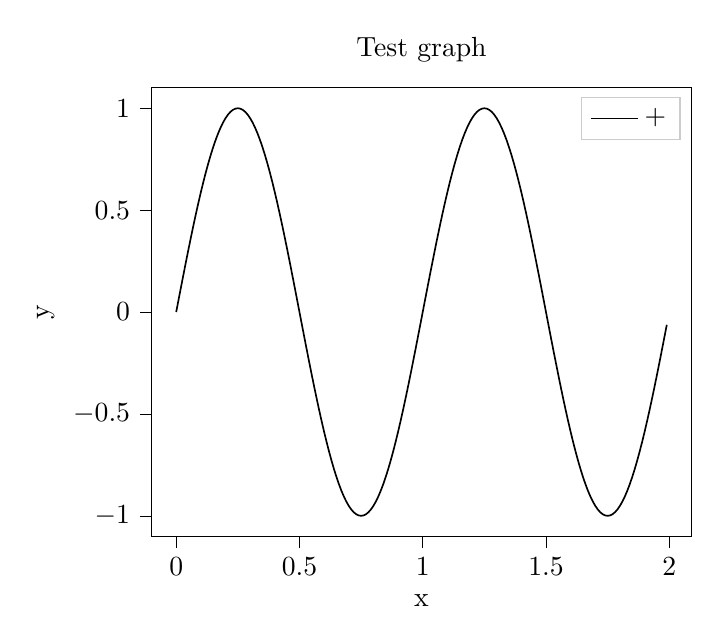
\begin{tikzpicture}

\definecolor{darkgray176}{RGB}{176,176,176}
\definecolor{lightgray204}{RGB}{204,204,204}

\begin{axis}[
legend cell align={left},
legend style={fill opacity=0.8, draw opacity=1, text opacity=1, draw=lightgray204},
tick align=outside,
tick pos=left,
title={Test graph},
x grid style={darkgray176},
xlabel={x},
xmin=-0.0995, xmax=2.0895,
xtick style={color=black},
y grid style={darkgray176},
ylabel={y},
ymin=-1.1, ymax=1.1,
ytick style={color=black}
]
\addplot [semithick, black]
table {%
0 0
0.01 0.0627905195293134
0.02 0.125333233564304
0.03 0.187381314585725
0.04 0.248689887164855
0.05 0.309016994374947
0.06 0.368124552684678
0.07 0.425779291565073
0.08 0.481753674101715
0.09 0.535826794978997
0.1 0.587785252292473
0.11 0.63742398974869
0.12 0.684547105928689
0.13 0.728968627421412
0.14 0.770513242775789
0.15 0.809016994374947
0.16 0.844327925502015
0.17 0.876306680043864
0.18 0.90482705246602
0.19 0.929776485888251
0.2 0.951056516295154
0.21 0.968583161128631
0.22 0.982287250728689
0.23 0.992114701314478
0.24 0.998026728428272
0.25 1
0.26 0.998026728428272
0.27 0.992114701314478
0.28 0.982287250728689
0.29 0.968583161128631
0.3 0.951056516295154
0.31 0.929776485888251
0.32 0.904827052466019
0.33 0.876306680043863
0.34 0.844327925502015
0.35 0.809016994374947
0.36 0.770513242775789
0.37 0.728968627421411
0.38 0.684547105928689
0.39 0.63742398974869
0.4 0.587785252292473
0.41 0.535826794978997
0.42 0.481753674101716
0.43 0.425779291565073
0.44 0.368124552684678
0.45 0.309016994374948
0.46 0.248689887164855
0.47 0.187381314585725
0.48 0.125333233564305
0.49 0.0627905195293136
0.5 1.22464679914735e-16
0.51 -0.0627905195293133
0.52 -0.125333233564304
0.53 -0.187381314585725
0.54 -0.248689887164855
0.55 -0.309016994374948
0.56 -0.368124552684678
0.57 -0.425779291565073
0.58 -0.481753674101715
0.59 -0.535826794978996
0.6 -0.587785252292473
0.61 -0.63742398974869
0.62 -0.684547105928689
0.63 -0.728968627421411
0.64 -0.770513242775789
0.65 -0.809016994374947
0.66 -0.844327925502015
0.67 -0.876306680043864
0.68 -0.90482705246602
0.69 -0.929776485888251
0.7 -0.951056516295154
0.71 -0.968583161128631
0.72 -0.982287250728689
0.73 -0.992114701314478
0.74 -0.998026728428272
0.75 -1
0.76 -0.998026728428272
0.77 -0.992114701314478
0.78 -0.982287250728689
0.79 -0.968583161128631
0.8 -0.951056516295154
0.81 -0.929776485888251
0.82 -0.90482705246602
0.83 -0.876306680043863
0.84 -0.844327925502016
0.85 -0.809016994374948
0.86 -0.77051324277579
0.87 -0.728968627421412
0.88 -0.684547105928689
0.89 -0.63742398974869
0.9 -0.587785252292473
0.91 -0.535826794978996
0.92 -0.481753674101715
0.93 -0.425779291565072
0.94 -0.368124552684678
0.95 -0.309016994374948
0.96 -0.248689887164855
0.97 -0.187381314585725
0.98 -0.125333233564305
0.99 -0.0627905195293133
1 -2.44929359829471e-16
1.01 0.0627905195293128
1.02 0.125333233564304
1.03 0.187381314585724
1.04 0.248689887164855
1.05 0.309016994374947
1.06 0.368124552684678
1.07 0.425779291565073
1.08 0.481753674101716
1.09 0.535826794978997
1.1 0.587785252292474
1.11 0.63742398974869
1.12 0.684547105928689
1.13 0.728968627421412
1.14 0.770513242775789
1.15 0.809016994374948
1.16 0.844327925502015
1.17 0.876306680043863
1.18 0.904827052466019
1.19 0.929776485888251
1.2 0.951056516295154
1.21 0.968583161128631
1.22 0.982287250728689
1.23 0.992114701314478
1.24 0.998026728428272
1.25 1
1.26 0.998026728428272
1.27 0.992114701314478
1.28 0.982287250728689
1.29 0.968583161128631
1.3 0.951056516295154
1.31 0.929776485888252
1.32 0.904827052466019
1.33 0.876306680043863
1.34 0.844327925502015
1.35 0.809016994374948
1.36 0.770513242775789
1.37 0.728968627421411
1.38 0.684547105928688
1.39 0.63742398974869
1.4 0.587785252292473
1.41 0.535826794978997
1.42 0.481753674101716
1.43 0.425779291565074
1.44 0.368124552684678
1.45 0.309016994374948
1.46 0.248689887164855
1.47 0.187381314585726
1.48 0.125333233564304
1.49 0.0627905195293134
1.5 3.67394039744206e-16
1.51 -0.0627905195293127
1.52 -0.125333233564303
1.53 -0.187381314585725
1.54 -0.248689887164855
1.55 -0.309016994374947
1.56 -0.368124552684677
1.57 -0.425779291565073
1.58 -0.481753674101716
1.59 -0.535826794978997
1.6 -0.587785252292473
1.61 -0.637423989748691
1.62 -0.684547105928689
1.63 -0.728968627421412
1.64 -0.770513242775789
1.65 -0.809016994374947
1.66 -0.844327925502016
1.67 -0.876306680043863
1.68 -0.904827052466019
1.69 -0.929776485888251
1.7 -0.951056516295153
1.71 -0.968583161128631
1.72 -0.982287250728688
1.73 -0.992114701314478
1.74 -0.998026728428272
1.75 -1
1.76 -0.998026728428272
1.77 -0.992114701314478
1.78 -0.982287250728689
1.79 -0.968583161128631
1.8 -0.951056516295154
1.81 -0.929776485888252
1.82 -0.904827052466019
1.83 -0.876306680043863
1.84 -0.844327925502015
1.85 -0.809016994374948
1.86 -0.770513242775789
1.87 -0.728968627421411
1.88 -0.684547105928689
1.89 -0.63742398974869
1.9 -0.587785252292473
1.91 -0.535826794978996
1.92 -0.481753674101716
1.93 -0.425779291565074
1.94 -0.368124552684678
1.95 -0.309016994374948
1.96 -0.248689887164856
1.97 -0.187381314585726
1.98 -0.125333233564304
1.99 -0.0627905195293135
};
\addlegendentry{+}
\end{axis}

\end{tikzpicture}
}}
	\caption{MIFA Antenna Gain Radiation Pattren}
\end{figure}